\documentclass[11pt,a4paper]{article}

% ---------------------------------------------------------------------
% Préambule
% ---------------------------------------------------------------------
\usepackage[utf8]{inputenc}
\usepackage[T1]{fontenc}
\usepackage[french,provide=*]{babel}
\usepackage{amsmath,amssymb,amsthm}
\usepackage{booktabs}
\usepackage{array}
\usepackage{geometry}
\usepackage{enumitem}
\usepackage{graphicx}
\usepackage{hyperref}
\usepackage{xcolor} % à ajouter si pas déjà présent
\hypersetup{
    colorlinks=true,
    linkcolor=blue,      % liens internes (sections, équations)
    citecolor=blue,      % citations bibliographiques [1], [2]
    urlcolor=blue        % liens web
}
\geometry{hmargin=1.7cm, vmargin=1.5cm}
\setlength{\parskip}{0.6em}
\setlength{\parindent}{0pt}
\renewcommand{\arraystretch}{1.25}
\setcounter{MaxMatrixCols}{13} % la matrice A a 13 colonnes (une par conduite)

% Environnements de théorème, en noir et blanc, sans couleur.
\theoremstyle{plain}
\newtheorem{theoreme}{Théorème}
\newtheorem{proposition}{Proposition}
\newtheorem{corollaire}{Corollaire}
\theoremstyle{definition}
\newtheorem{definition}{Définition}
\theoremstyle{remark}
\newtheorem{remarque}{Remarque}

\title{\textbf{Représentation algébrique du réseau}}
\date{}
\begin{document}
\maketitle
\vspace{-4em}

\begin{abstract}
\noindent
Cette section traduit algébriquement le réseau fixé par le Membre 1 : à
partir du graphe $G=(V,E)$ et de sa matrice d'incidence orientée $A$, on
établit le rang de $A$, la dimension de son noyau, et le conditionnement de
$A$ et de $A^\top A$. Ces résultats jouent un double rôle dans le projet :
d'une part ils garantissent que le système de conservation des flux
$Aq = b$ est bien posé sur le réseau étudié, d'autre part le
conditionnement de $A^\top A$ fixe, pour le Membre 4, la borne théorique sur
le pas d'apprentissage de la descente de gradient.
\end{abstract}

\section{Cadre et notations}

Le réseau est représenté par un graphe orienté connexe $G = (V, E)$, où
$V = V_R \cup V_Q$ regroupe les $n_R = 2$ réservoirs $\{R_1, R_2\}$ et les
$n_Q = 8$ quartiers $\{Q_1, \dots, Q_8\}$, soit $n = |V| = 10$ nœuds, et où
$E$ désigne l'ensemble des $m = |E| = 13$ conduites. Cette topologie, ainsi
que l'orientation de référence de chaque conduite, ont été fixées et
justifiées par le Membre 1 ; elles ne sont pas remises en cause ici, mais
traduites sous forme matricielle.

Pour la construction de $A$, les nœuds et les arêtes sont numérotés dans
l'ordre fixé par le Membre 1 (réservoirs d'abord, puis quartiers dans
l'ordre $Q_1, \dots, Q_8$ ; conduites $e_1, \dots, e_{13}$ dans l'ordre du
fichier de configuration), rappelé au Tableau~\ref{tab:indexation}.

\begin{table}[h]
\centering
\begin{tabular}{@{}ll@{}}
\toprule
Indice de ligne & Nœud \\
\midrule
1 -- 2 & $R_1$, $R_2$ (réservoirs) \\
3 -- 10 & $Q_1, Q_2, \dots, Q_8$ (quartiers) \\
\bottomrule
\end{tabular}
\qquad
\begin{tabular}{@{}ll@{}}
\toprule
Arête & Conduite \\
\midrule
$e_1$ & $R_1 \to Q_1$ \\
$e_2$ & $R_1 \to Q_2$ \\
$e_3$ & $Q_2 \to Q_3$ \\
$e_4$ & $Q_3 \to Q_4$ \\
$e_5$ & $R_2 \to Q_5$ \\
$e_6$ & $R_2 \to Q_6$ \\
$e_7$ & $Q_6 \to Q_7$ \\
\bottomrule
\end{tabular}
\qquad
\begin{tabular}{@{}ll@{}}
\toprule
Arête & Conduite \\
\midrule
$e_8$ & $Q_7 \to Q_8$ \\
$e_9$ & $Q_4 \to Q_5$ \\
$e_{10}$ & $Q_3 \to Q_6$ \\
$e_{11}$ & $Q_2 \to Q_4$ \\
$e_{12}$ & $Q_5 \to Q_6$ \\
$e_{13}$ & $Q_6 \to Q_8$ \\
& \\
\bottomrule
\end{tabular}
\caption{Indexation de référence des nœuds (lignes de $A$) et des arêtes
(colonnes de $A$), reprise de la structure de données de M1.}
\label{tab:indexation}
\end{table}

\section{Construction de la matrice d'incidence}

\begin{definition}[Matrice d'incidence orientée]
Pour un graphe orienté $G = (V, E)$ à $n$ nœuds et $m$ arêtes, la matrice
d'incidence $A \in \mathbb{R}^{n \times m}$ est définie, pour chaque nœud
$i \in V$ et chaque arête $e = (u, v) \in E$, par
\begin{equation}
A_{i e} =
\begin{cases}
-1 & \text{si } i = u \text{ (nœud de départ de } e \text{)}, \\
+1 & \text{si } i = v \text{ (nœud d'arrivée de } e \text{)}, \\
\phantom{-}0 & \text{sinon.}
\end{cases}
\label{eq:def-A}
\end{equation}
\end{definition}

Cette convention est celle retenue par M1 pour orienter chaque conduite
(des réservoirs vers la périphérie du réseau) et pour interpréter physiquement
$Aq = b$. Avec cette convention, pour tout vecteur de débit
$q \in \mathbb{R}^m$, la $i$-ième composante de $Aq$ vaut
\begin{equation}
(Aq)_i \;=\; \sum_{e \,=\, (\cdot,\, i)} q_e \;-\; \sum_{e \,=\, (i,\, \cdot)} q_e,
\label{eq:Aq-i}
\end{equation}
c'est-à-dire la somme des débits \emph{entrant} au nœud $i$ moins la somme
des débits \emph{sortant} de $i$ : le débit net entrant. La contrainte
$Aq = b$, avec
\[
b = \big(-s(R_1),\, -s(R_2),\, D_1, \dots, D_8\big)^\top \in \mathbb{R}^{10},
\]
exprime alors, nœud par nœud, la conservation de la matière : aux
réservoirs, le débit net sortant égale l'offre injectée ; aux quartiers, le
débit net entrant égale la demande à satisfaire.

En appliquant \eqref{eq:def-A} à chacune des 13 conduites du réseau selon
l'ordre du Tableau~\ref{tab:indexation}, on obtient la matrice d'incidence
complète du réseau :

\begin{equation}
A =
\begin{pmatrix}
-1 & -1 &  0 &  0 &  0 &  0 &  0 &  0 &  0 &  0 &  0 &  0 &  0 \\
 0 &  0 &  0 &  0 & -1 & -1 &  0 &  0 &  0 &  0 &  0 &  0 &  0 \\
+1 &  0 &  0 &  0 &  0 &  0 &  0 &  0 &  0 &  0 &  0 &  0 &  0 \\
 0 & +1 & -1 &  0 &  0 &  0 &  0 &  0 &  0 &  0 & -1 &  0 &  0 \\
 0 &  0 & +1 & -1 &  0 &  0 &  0 &  0 &  0 & -1 &  0 &  0 &  0 \\
 0 &  0 &  0 & +1 &  0 &  0 &  0 &  0 & -1 &  0 & +1 &  0 &  0 \\
 0 &  0 &  0 &  0 & +1 &  0 &  0 &  0 & +1 &  0 &  0 & -1 &  0 \\
 0 &  0 &  0 &  0 &  0 & +1 & -1 &  0 &  0 & +1 &  0 & +1 & -1 \\
 0 &  0 &  0 &  0 &  0 &  0 & +1 & -1 &  0 &  0 &  0 &  0 &  0 \\
 0 &  0 &  0 &  0 &  0 &  0 &  0 & +1 &  0 &  0 &  0 &  0 & +1
\end{pmatrix}
\begin{array}{l}
R_1 \\ R_2 \\ Q_1 \\ Q_2 \\ Q_3 \\ Q_4 \\ Q_5 \\ Q_6 \\ Q_7 \\ Q_8
\end{array}
\label{eq:matrice-A}
\end{equation}

\begin{remarque}
Chaque colonne de $A$ contient exactement un $-1$ et un $+1$ : c'est une
conséquence directe de la définition \eqref{eq:def-A}, puisqu'une arête a
exactement un nœud de départ et un nœud d'arrivée. Cette propriété, en
apparence anodine, est en réalité le point de départ de toute la Section
\ref{sec:rang} : elle implique que la somme des lignes de $A$ est
identiquement nulle.
\end{remarque}

\section{Rang de la matrice d'incidence et connexité}
\label{sec:rang}

Le rang de $A$ détermine si le système $Aq = b$ admet une solution
cohérente sur l'ensemble du réseau, et de combien de degrés de liberté on
dispose pour la choisir. On démontre ici le résultat classique reliant ce
rang à la connexité du graphe~\cite{godsil2001,diestel2010}, puis on le
vérifie sur le réseau concret de M1.

\begin{theoreme}[Rang de la matrice d'incidence d'un graphe connexe]
Soit $G = (V, E)$ un graphe orienté à $n = |V|$ nœuds, connexe (au sens
non orienté), et soit $A \in \mathbb{R}^{n \times m}$ sa matrice
d'incidence. Alors
\begin{equation}
\operatorname{rg}(A) = n - 1.
\label{eq:rang-theoreme}
\end{equation}
\end{theoreme}

\begin{proof}
La démonstration se fait en deux temps : on montre d'abord que
$\operatorname{rg}(A) \le n - 1$, puis que cette borne est atteinte.

\medskip
\noindent\textit{Étape 1 --- $\operatorname{rg}(A) \le n-1$.}
Soit $\mathbf{1} = (1, 1, \dots, 1)^\top \in \mathbb{R}^n$ le vecteur dont
toutes les composantes valent $1$. Pour toute arête $e \in E$, la colonne
de $A$ associée à $e$ contient exactement un $-1$ et un $+1$ (le reste
étant nul), donc la somme des composantes de cette colonne vaut
\[
\sum_{i=1}^{n} A_{ie} = (-1) + (+1) = 0.
\]
Ceci vaut pour \emph{chaque} colonne $e = 1, \dots, m$, ce qui s'écrit sous
forme matricielle
\begin{equation}
\mathbf{1}^\top A = \mathbf{0}^\top.
\label{eq:1TA}
\end{equation}
L'égalité \eqref{eq:1TA} signifie que $\mathbf{1}$ appartient au noyau à
gauche de $A$, c'est-à-dire $\mathbf{1} \in \ker(A^\top)$, avec
$\mathbf{1} \ne \mathbf{0}$. Les $n$ lignes de $A$ sont donc linéairement
dépendantes, d'où
\begin{equation}
\operatorname{rg}(A) = \operatorname{rg}(A^\top) \le n - 1.
\label{eq:etape1}
\end{equation}

\medskip
\noindent\textit{Étape 2 --- $\operatorname{rg}(A) \ge n-1$, via
$\dim \ker(A^\top) \le 1$.}
Réciproquement, soit $x \in \mathbb{R}^n$ un vecteur quelconque du noyau à
gauche, $A^\top x = 0$. Pour toute arête $e = (u, v) \in E$, la ligne de
$A^\top x = 0$ correspondant à $e$ s'écrit, d'après la définition
\eqref{eq:def-A} de $A$,
\[
(A^\top x)_e = A_{ue}\, x_u + A_{ve}\, x_v = (-1)\, x_u + (+1)\, x_v = x_v - x_u = 0,
\]
c'est-à-dire
\begin{equation}
x_u = x_v \qquad \text{pour toute arête } (u,v) \in E.
\label{eq:xu-xv}
\end{equation}
La relation \eqref{eq:xu-xv} dit que $x$ est constant le long de toute
arête. Comme $G$ est connexe, deux nœuds quelconques $i$ et $j$ sont reliés
par une chaîne $i = k_0, k_1, \dots, k_p = j$ où chaque paire
$(k_{\ell-1}, k_\ell)$ correspond à une arête du graphe non orienté sous-jacent.
En appliquant \eqref{eq:xu-xv} le long de cette chaîne, par transitivité,
\[
x_{k_0} = x_{k_1} = \cdots = x_{k_p}, \qquad \text{donc } x_i = x_j.
\]
Ceci valant pour tout couple $(i,j)$, toutes les composantes de $x$ sont
égales : $x = \alpha \, \mathbf{1}$ pour un certain $\alpha \in \mathbb{R}$.
Autrement dit,
\begin{equation}
\ker(A^\top) = \operatorname{vect}(\mathbf{1}), \qquad \dim \ker(A^\top) = 1.
\label{eq:dim-ker-AT}
\end{equation}

\medskip
\noindent\textit{Conclusion.} Par le théorème du rang appliqué à
$A^\top \in \mathbb{R}^{m \times n}$ (vu comme application linéaire de
$\mathbb{R}^n$ dans $\mathbb{R}^m$),
\[
\operatorname{rg}(A^\top) = n - \dim \ker(A^\top) \overset{\eqref{eq:dim-ker-AT}}{=} n - 1.
\]
Comme $\operatorname{rg}(A) = \operatorname{rg}(A^\top)$ (le rang d'une
matrice est égal au rang de sa transposée), on obtient
$\operatorname{rg}(A) = n - 1$, ce qui, combiné à \eqref{eq:etape1},
achève la démonstration.
\end{proof}

\begin{remarque}
La démonstration montre en réalité un résultat plus fin que le seul énoncé
du théorème : $\dim \ker(A^\top) = 1$ exactement (et non seulement
$\le 1$) est \emph{équivalent} à la connexité de $G$. Si $G$ avait $k$
composantes connexes, le même raisonnement appliqué à chaque composante
donnerait $\dim \ker(A^\top) = k$ et $\operatorname{rg}(A) = n - k$. Le
rang de $A$ mesure donc exactement le nombre de composantes connexes du
réseau.
\end{remarque}

\paragraph{Application au réseau de M1.}
Le réseau construit par le Membre 1 comporte $n = 10$ nœuds et a été
vérifié connexe (une seule composante connexe, comme indiqué dans son
document de topologie). Le Théorème 1 prédit donc
\begin{equation}
\operatorname{rg}(A) = n - 1 = 10 - 1 = 9.
\end{equation}
Ce résultat est vérifié numériquement par le calcul du rang de la matrice
\eqref{eq:matrice-A} (module \texttt{graph\_analysis.py}, fonctions
\texttt{est\_connexe} et \texttt{rang}) : le rang effectif calculé sur $A$
est bien $9$, en accord exact avec la prédiction théorique.

\section{Noyau de la matrice d'incidence et cycles indépendants}

Le rang ne renseigne que sur la dimension de l'image de $A$ ; la dimension
de son noyau renseigne, elle, sur le nombre de degrés de liberté dont
dispose l'algorithme d'optimisation pour répartir les débits sans violer la
conservation des flux : c'est précisément ce que quantifient les cycles du
réseau.

\begin{corollaire}[Dimension du noyau de $A$]
Avec les notations précédentes,
\begin{equation}
\dim \ker(A) = m - \operatorname{rg}(A) = m - n + 1.
\label{eq:dim-ker-A}
\end{equation}
\end{corollaire}

\begin{proof}
Conséquence immédiate du théorème du rang appliqué à $A$, vue comme
application linéaire de $\mathbb{R}^m$ dans $\mathbb{R}^n$ :
$\operatorname{rg}(A) + \dim \ker(A) = m$, d'où
$\dim \ker(A) = m - \operatorname{rg}(A)$, qui vaut $m - n + 1$ d'après le
Théorème 1.
\end{proof}

\paragraph{Application au réseau de M1.} Avec $m = 13$ et $n = 10$,
\begin{equation}
\dim \ker(A) = 13 - 9 = 4.
\end{equation}
Le réseau possède donc exactement 4 cycles indépendants (nombre
cyclomatique du graphe~\cite{bapat2010}). Une base explicite de ces 4
cycles s'obtient en choisissant un arbre couvrant du réseau, par exemple
constitué des 8 conduites de backbone ($e_1$ à $e_8$) complétées par la
conduite inter-zones $e_{10}$ ($Q_3 \to Q_6$), soit $9 = n-1$ arêtes
formant un arbre. Les $4 = m - (n-1)$ conduites restantes ($e_9$, $e_{11}$,
$e_{12}$, $e_{13}$) sont les \emph{arêtes de chaînage} (ou \emph{chords}) de
cet arbre : chacune, ajoutée à l'arbre, referme exactement un cycle. Ces
quatre cycles fondamentaux sont donnés au Tableau~\ref{tab:cycles} ; la
fonction \texttt{noyau} du module \texttt{graph\_analysis.py} calcule quant
à elle une base orthonormée du même sous-espace par décomposition en
valeurs singulières, numériquement plus robuste mais moins directement
lisible en termes de cycles.

\begin{table}[h]
\centering
\begin{tabular}{@{}lll@{}}
\toprule
Arête de chaînage & Cycle fondamental correspondant & Longueur \\
\midrule
$e_{11}$ ($Q_2 \to Q_4$) & $Q_2 - Q_3 - Q_4 - Q_2$ & 3 arêtes \\
$e_{13}$ ($Q_6 \to Q_8$) & $Q_6 - Q_7 - Q_8 - Q_6$ & 3 arêtes \\
$e_{12}$ ($Q_5 \to Q_6$) & $Q_5 - R_2 - Q_6 - Q_5$ & 3 arêtes \\
$e_{9}$ ($Q_4 \to Q_5$) & $Q_4 - Q_3 - Q_6 - R_2 - Q_5 - Q_4$ & 5 arêtes \\
\bottomrule
\end{tabular}
\caption{Base des 4 cycles indépendants du réseau, obtenue par la méthode
de l'arbre couvrant. Chaque cycle correspond à une boucle de secours
identifiée par M1 dans sa justification de topologie.}
\label{tab:cycles}
\end{table}

Les trois premiers cycles coïncident avec les trois boucles de redondance
identifiées par M1 ($Q_2$--$Q_4$, $Q_5$--$Q_6$, $Q_6$--$Q_8$) ; le
quatrième correspond aux deux connexions inter-zones ($e_9$, $e_{10}$),
qui à elles deux referment un cycle traversant l'ensemble du réseau.

\section{Points de fragilité}
\label{sec:ponts}

Trois notions distinctes de fragilité structurelle sont formalisées ici,
toutes définies sur le graphe non orienté sous-jacent (l'orientation des
conduites étant une convention de modélisation pour $A$, non une contrainte
physique sur la propagation d'une panne) : les nœuds de degré 1, les
arêtes-ponts, et les points d'articulation.

\begin{definition}[Pont]
Dans un graphe non orienté connexe $G = (V,E)$, une arête $e \in E$ est un
\emph{pont} si le graphe $G - e$ (obtenu en supprimant $e$) n'est plus
connexe.
\end{definition}

\begin{proposition}
Une arête $e = (u,v)$ est un pont si et seulement si elle n'appartient à
aucun cycle de $G$.
\end{proposition}

\begin{proof}
Si $e$ appartient à un cycle $C$, alors pour tout couple de nœuds
initialement reliés par un chemin passant par $e$, ce chemin peut être
détourné en empruntant le reste du cycle $C \setminus \{e\}$ : $G - e$
reste donc connexe, et $e$ n'est pas un pont. Réciproquement, si $e$
n'appartient à aucun cycle, alors $e$ est la seule arête reliant les deux
sous-graphes obtenus en supprimant $e$ (sans quoi elles formeraient, avec
$e$, un cycle) ; $G - e$ est donc déconnecté et $e$ est un pont.
\end{proof}

Cette caractérisation relie directement la notion de pont à celle de cycle
étudiée à la section précédente : une arête absente de toute base de
cycles (Tableau~\ref{tab:cycles}) est nécessairement un pont, puisque les
arêtes d'un arbre couvrant n'appartiennent, par construction, à aucun
cycle tant que les arêtes de chaînage ne sont pas incluses.

\begin{definition}[Point d'articulation]
Dans un graphe non orienté connexe $G = (V,E)$, un nœud $v \in V$ est un
\emph{point d'articulation} si le graphe $G - v$ (obtenu en supprimant $v$
et toutes les arêtes qui lui sont incidentes) n'est plus connexe.
\end{definition}

Un pont prive potentiellement plusieurs quartiers d'eau simultanément (tout
un sous-arbre en aval) ; un nœud de degré 1 n'affecte que lui-même ; un
point d'articulation généralise le pont à la suppression d'un nœud plutôt
que d'une arête, et peut isoler plusieurs branches à la fois si son degré
est supérieur à 2.

\paragraph{Application au réseau de M1.} Les trois fonctions de
\texttt{detecter\_points\_de\_fragilite} (module \texttt{graph\_analysis.py},
appuyées sur la bibliothèque \texttt{networkx}) donnent, sur le réseau de
M1 :
\begin{itemize}[nosep]
\item nœuds de degré 1 : $\{Q_1\}$ ;
\item arêtes-ponts : $\{(R_1,Q_1),\ (R_1,Q_2)\}$ ;
\item points d'articulation : $\{R_1,\ Q_2,\ Q_6\}$.
\end{itemize}
$R_1$ n'a que deux voisins, $Q_1$ (degré 1) et $Q_2$. En supprimant
$(R_1,Q_2)$, le sous-ensemble $\{R_1, Q_1\}$ ne conserve que l'arête
$(R_1,Q_1)$ et perd tout lien avec le reste du réseau : $(R_1,Q_2)$ est
donc un pont, au même titre que $(R_1,Q_1)$ ; le fichier de configuration
de M1 ne signalait que ce dernier. $Q_2$ et $Q_6$ apparaissent comme
points d'articulation car ce sont les deux seuls nœuds par lesquels
transitent, respectivement, la branche $Q_1$ et l'ensemble de la zone
$R_2$ ($Q_5$ à $Q_8$) : leur retrait déconnecterait ces branches du reste
du réseau, même si aucune conduite individuelle incidente à $Q_2$ ou $Q_6$
n'est elle-même un pont (hormis $(R_1,Q_2)$, déjà comptée).

\section{Conditionnement de $A$ et de $A^\top A$}

Le conditionnement quantifie la sensibilité numérique de la résolution
d'un système linéaire (ou, ici, d'un problème d'optimisation quadratique)
aux erreurs d'arrondi et à la structure du réseau.

\begin{definition}[Conditionnement effectif]
$A$ n'étant pas de rang plein colonne dès que $\dim \ker(A) > 0$ (ce qui
est le cas ici, Section 4), sa plus petite valeur singulière au sens
strict est nulle et le conditionnement usuel $\sigma_{\max}/\sigma_{\min}$
serait infini. On définit donc le \emph{conditionnement effectif}, restreint
au sous-espace orthogonal au noyau, comme le rapport de la plus grande à la
plus petite valeur singulière (resp. propre) \emph{strictement positive} :
\begin{equation}
\kappa(A) = \frac{\sigma_{\max}(A)}{\sigma_{\min}^{+}(A)}, \qquad
\kappa(A^\top A) = \frac{\lambda_{\max}(A^\top A)}{\lambda_{\min}^{+}(A^\top A)},
\end{equation}
où $\sigma_{\min}^{+}$ (resp. $\lambda_{\min}^{+}$) désigne la plus petite
valeur singulière (resp. propre) strictement positive. Comme $A^\top A$ est
symétrique positive, ses valeurs propres sont les carrés des valeurs
singulières de $A$, donc $\kappa(A^\top A) = \kappa(A)^2$.
\end{definition}

\paragraph{Pourquoi ce conditionnement importe pour M4.} La fonction de
coût pénalisée de M4 s'écrit $J(q) = q^\top C q + \mu \|Aq - b\|^2$, avec
$C = \operatorname{diag}(c_e)$. Son Hessien vaut $H = 2C + 2\mu A^\top A$,
et sa plus grande valeur propre est la constante de Lipschitz $L$ du
gradient, qui fixe la borne théorique sur le pas d'apprentissage
$\eta < 2/L$. Le module \texttt{graph\_analysis.py} distingue deux
fonctions : \texttt{conditionnement}, qui calcule $\kappa(A)$ seul
(propriété intrinsèque du graphe, indépendante de $c_e$ et $\mu$, utilisée
à l'Expérience 5) et \texttt{constante\_de\_lipschitz}, qui calcule $L$
exactement une fois $c_e$ et $\mu$ fixés (quantité à transmettre à M4).

\paragraph{Application au réseau de M1.} Le calcul des valeurs
singulières de $A$ (fonction \texttt{conditionnement} du module
\texttt{graph\_analysis.py}) donne les neuf valeurs singulières strictement
positives suivantes, arrondies à quatre décimales :
\begin{equation}
\sigma(A) \approx \big(2.4998,\ 2.1400,\ 2.0000,\ 1.7937,\ 1.7321,\ 1.5588,\ 1.1704,\ 0.9349,\ 0.5291\big),
\end{equation}
et une dixième valeur singulière numériquement nulle, cohérente avec
$\dim \ker(A^\top) = 1$ (une seule composante connexe, Section~\ref{sec:rang}).
On en déduit
\begin{equation}
\kappa(A) = \frac{\sigma_{\max}(A)}{\sigma_{\min}^{+}(A)} = \frac{2.4998}{0.5291} \approx 4.72.
\end{equation}
Le spectre de $A^\top A$ comporte quatre valeurs propres numériquement
nulles (conformes à $\dim \ker(A) = 4$, Section 4) et neuf valeurs propres
strictement positives, dont
\begin{equation}
\lambda_{\min}^{+}(A^\top A) \approx 0.2800, \qquad
\lambda_{\max}(A^\top A) \approx 6.2490,
\end{equation}
ce qui donne
\begin{equation}
\kappa(A^\top A) = \frac{\lambda_{\max}(A^\top A)}{\lambda_{\min}^{+}(A^\top A)} \approx \frac{6.2490}{0.2800} \approx 22.32,
\end{equation}
en accord avec $\kappa(A^\top A) = \kappa(A)^2 \approx 4.72^2 \approx 22.29$
(écart résiduel dû à l'arrondi des valeurs intermédiaires). $\lambda_{\max}(A^\top A) \approx 6.25$
est la quantité intrinsèque au graphe, indépendante de $\mu$, utilisée pour
comparer les variantes de maillage. La quantité exacte transmise à M4 est
$L(\mu) = \lambda_{\max}(2C + 2\mu A^\top A)$, calculée par
\texttt{constante\_de\_lipschitz} : par exemple, pour $\mu = 1$ sur le
réseau de M1, $L \approx 14.95$, d'où un pas recommandé
$\eta < 2/L \approx 0.134$.

\section{Lien entre maillage et conditionnement}

\begin{proposition}[Effet qualitatif du maillage]
Toutes choses égales par ailleurs (même nombre de nœuds, mêmes capacités
et coûts sur les arêtes communes), un réseau plus densément maillé --- au
sens où l'on ajoute des conduites transversales reliant des nœuds déjà
connectés par un autre chemin --- tend à réduire le conditionnement
$\kappa(A^\top A)$, ou au pire à le laisser inchangé.
\end{proposition}

\begin{proof}[Argument]
Ajouter une conduite au réseau revient à ajouter une colonne à $A$. Cela
ne peut qu'augmenter (au sens large) le rang de l'ensemble des directions
couvertes par l'image de $A^\top$, et donc élargir l'ensemble des valeurs
singulières non nulles disponibles ; en particulier, cela ne peut que faire
croître (ou laisser inchangée) la plus petite valeur singulière strictement
positive $\sigma_{\min}^{+}(A)$, associée à la direction du réseau la
« moins bien reliée ». À l'inverse, un réseau proche d'un arbre couvrant
(peu de cycles, donc peu de chemins alternatifs) concentre l'essentiel du
transport sur un petit nombre de conduites-clés, ce qui produit des
valeurs singulières très inégales, donc un conditionnement élevé. Une
preuve quantitative complète dépasserait le cadre de cette section ; le
sens de variation qualitatif est confronté aux mesures numériques dans
l'Expérience 5 (Section 6 du rapport), où $\kappa(A^\top A)$ est mesuré
sur des variantes du réseau de densité croissante, de l'arbre couvrant
($4$ cycles supprimés) au réseau complet ($4$ cycles).
\end{proof}

\begin{remarque}
La Proposition 2 sera testée à l'Expérience 5 : mesure de
$\kappa(A^\top A)$ via la fonction \texttt{conditionnement}, appliquée à
des variantes du réseau de M1, de l'arbre couvrant au réseau complet.
\end{remarque}

\section{Synthèse des résultats transmis au reste du groupe}

\begin{table}[h]
\centering
\begin{tabular}{@{}llc@{}}
\toprule
Grandeur & Destinataire & Valeur \\
\midrule
$\operatorname{rg}(A)$ & Validation interne (M1, M2) & $9$ \\
$\dim \ker(A)$ (cycles indépendants) & M6 (Expérience 5) & $4$ \\
Ponts (points de fragilité) & M1, M6 (scénarios de panne) & $(R_1,Q_1)$, $(R_1,Q_2)$ \\
Points d'articulation & M1, M6 (scénarios de panne) & $R_1$, $Q_2$, $Q_6$ \\
$\lambda_{\max}(A^\top A)$ & M6 (Expérience 5) & $\approx 6.25$ \\
$\kappa(A^\top A)$ & M6 (Expérience 5) & $\approx 22.3$ \\
$L(\mu{=}1) = \lambda_{\max}(2C + 2A^\top A)$ & M4 (borne sur le pas $\eta$) & $\approx 14.95$ \\
\bottomrule
\end{tabular}
\caption{Résultats de la présente analyse et destinataires dans le
pipeline du projet.}
\end{table}
NB : Les calculs formels et la structure du document ont été vérifiés avec l'assistance de Claude~\cite{claude}.
\renewcommand{\refname}{Références bibliographiques}

\begin{thebibliography}{99}
\makeatletter
\def\@openbib@code{\itemsep=0.35em\parsep=0pt}
\makeatother

\bibitem{cours}
Ir.~Charbel Mamlankou, \emph{Mathématiques fondamentales pour l'IA}, support de cours, AMA, 2026.

\bibitem{web-incidence}
Wikipédia, \emph{Matrice d'incidence}. \href{https://fr.wikipedia.org/wiki/Matrice_d'incidence}{[Article en ligne]}.

\bibitem{video-graphes}
Ressources audiovisuelles sur les matrices d'incidence et connexité : 
\href{https://www.youtube.com/watch?v=c1m7L_fHLXU}{Tutoriel d'introduction} et 
\href{https://www.youtube.com/watch?v=PMWo9xweSEA}{Graphes et matrices d'incidence}.

\bibitem{claude}
Anthropic, \emph{Claude 3.5 Sonnet} [Grand modèle de langage], 2026. Disponible sur : \url{https://www.anthropic.com/claude}.
\end{thebibliography}

% ---------------------------------------------------------------------
% Annexes : Exécutions et Visualisation du réseau
% --------------------------------------------------------------------*
\appendix

\section{Résultats d'exécution du code et visualisation du graphe}
\label{sec:annexes-executions}

Cette annexe regroupe les sorties effectives des modules d'implémentation, validant numériquement l'ensemble des théorèmes et propriétés topologiques établis dans le document.

\subsection{Validation de la construction matricielle (\texttt{build\_graph.py})}

La commande \texttt{python3 -m src.graph.build\_graph} instancie le graphe orienté ($n=10$, $m=13$), assemble la matrice d'incidence $A \in \mathbb{R}^{10 \times 13}$ ainsi que le vecteur de coût $c_e$ et le second membre $b$.

\begin{figure}[htbp]
\centering
% Renommez votre 1re capture (terminal build_graph) en capture_build_graph.png
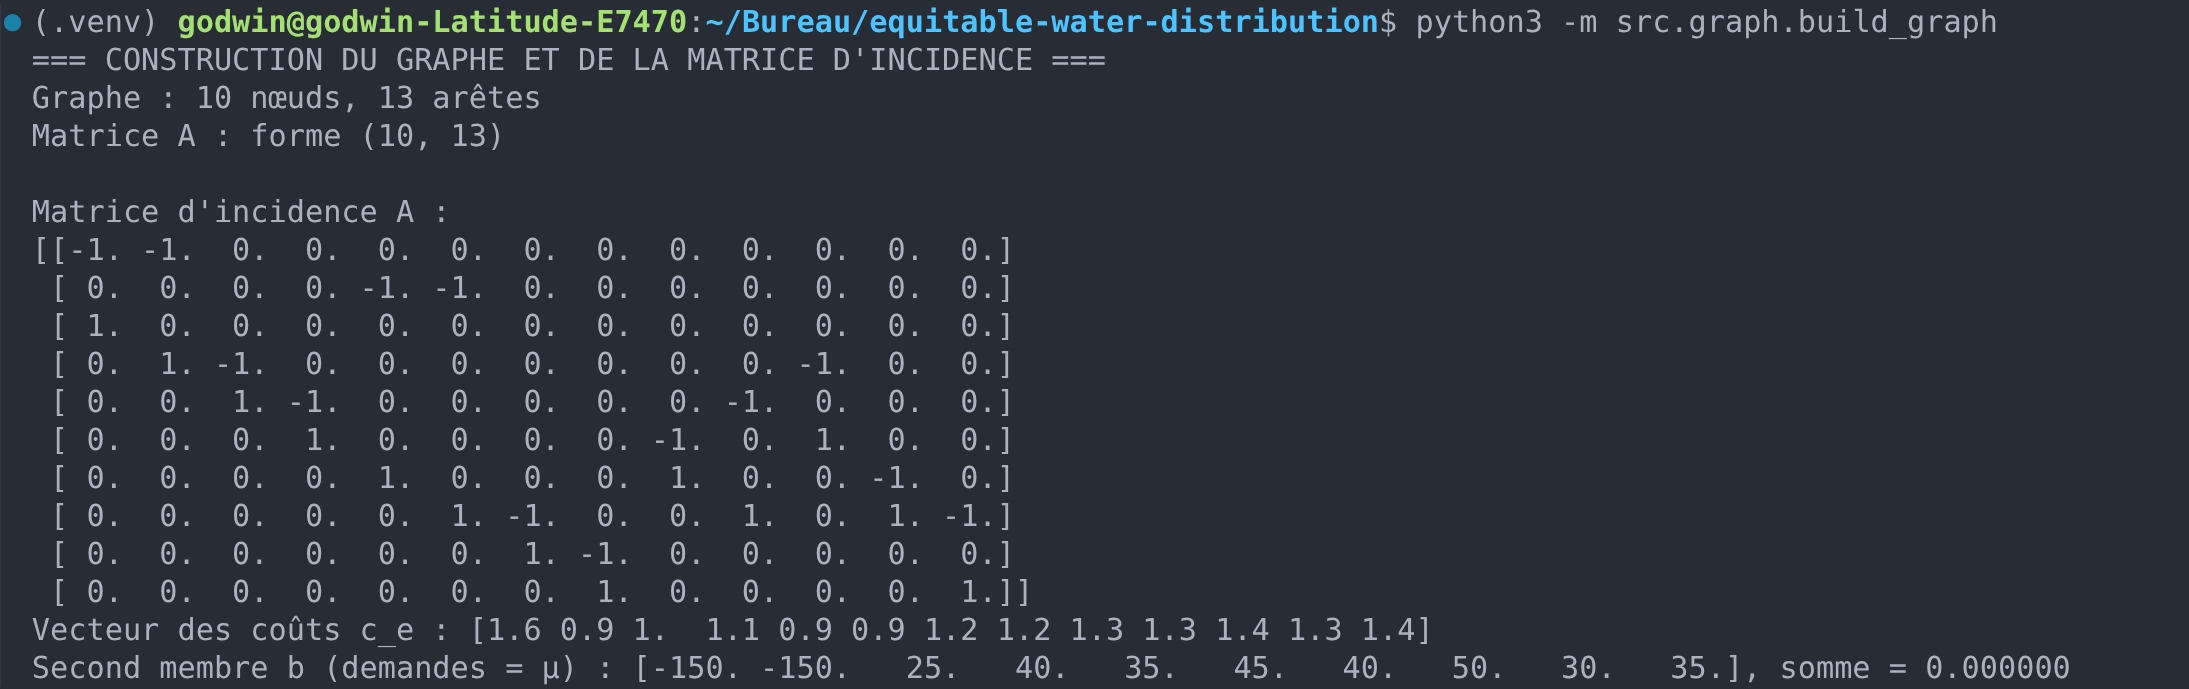
\includegraphics[width=\textwidth]{capture_build_graph.png}
\caption{Sortie terminal confirmant la structure de la matrice d'incidence $A$, le vecteur des coûts $c_e$ et la conservation globale $\sum b_i = 0$.}
\label{fig:exec-build}
\end{figure}

\subsection{Analyse spectrale et points de fragilité (\texttt{graph\_analysis.py})}

L'exécution du script \texttt{src.graph.graph\_analysis} corrobore l'ensemble des grandeurs théoriques : rang effectif $\operatorname{rg}(A) = 9$, dimension du noyau $\dim\ker(A) = 4$, conditionnement $\kappa(A) \approx 4.7244$, constante de Lipschitz $L(\mu=1.0) \approx 14.9525$, ainsi que la détection exacte des ponts et points d'articulation.

\begin{figure}[htbp]
\centering
% Renommez votre 2e capture (terminal graph_analysis) en capture_analysis.png
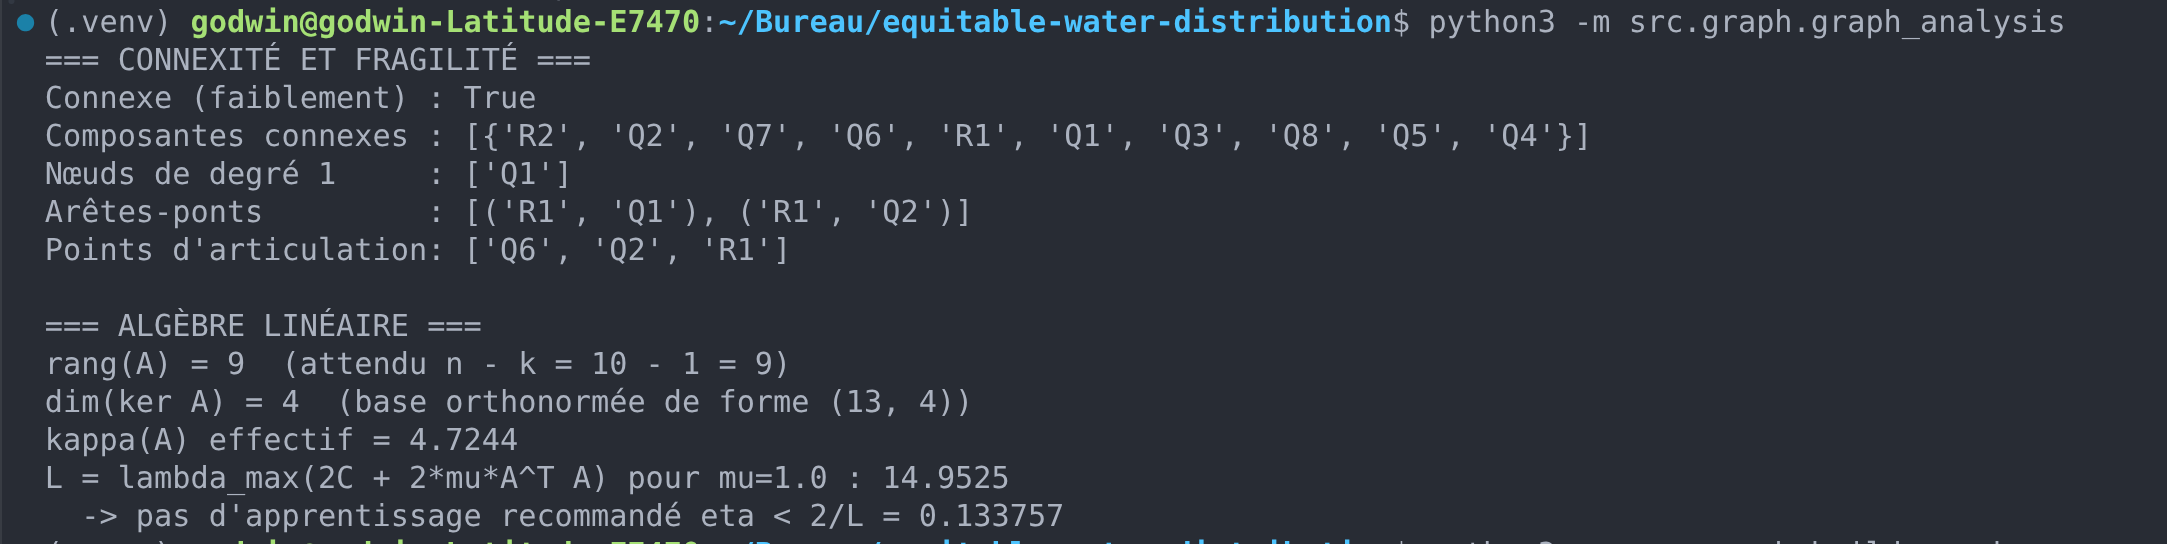
\includegraphics[width=\textwidth]{capture_analysis.png}
\caption{Validation numérique de la connexité, des points de fragilité, du rang, du conditionnement effectif et de la borne de Lipschitz $\eta < 0.133757$.}
\label{fig:exec-analysis}
\end{figure}

\clearpage
\subsection{Visualisation spatiale du réseau de distribution}

\begin{figure}[htbp]
\centering
% Renommez votre 3e capture (graphe avec nœuds bleus) en graphe_reseau.png
% Le trim permet de rogner les marges blanches : {gauche bas droite haut}
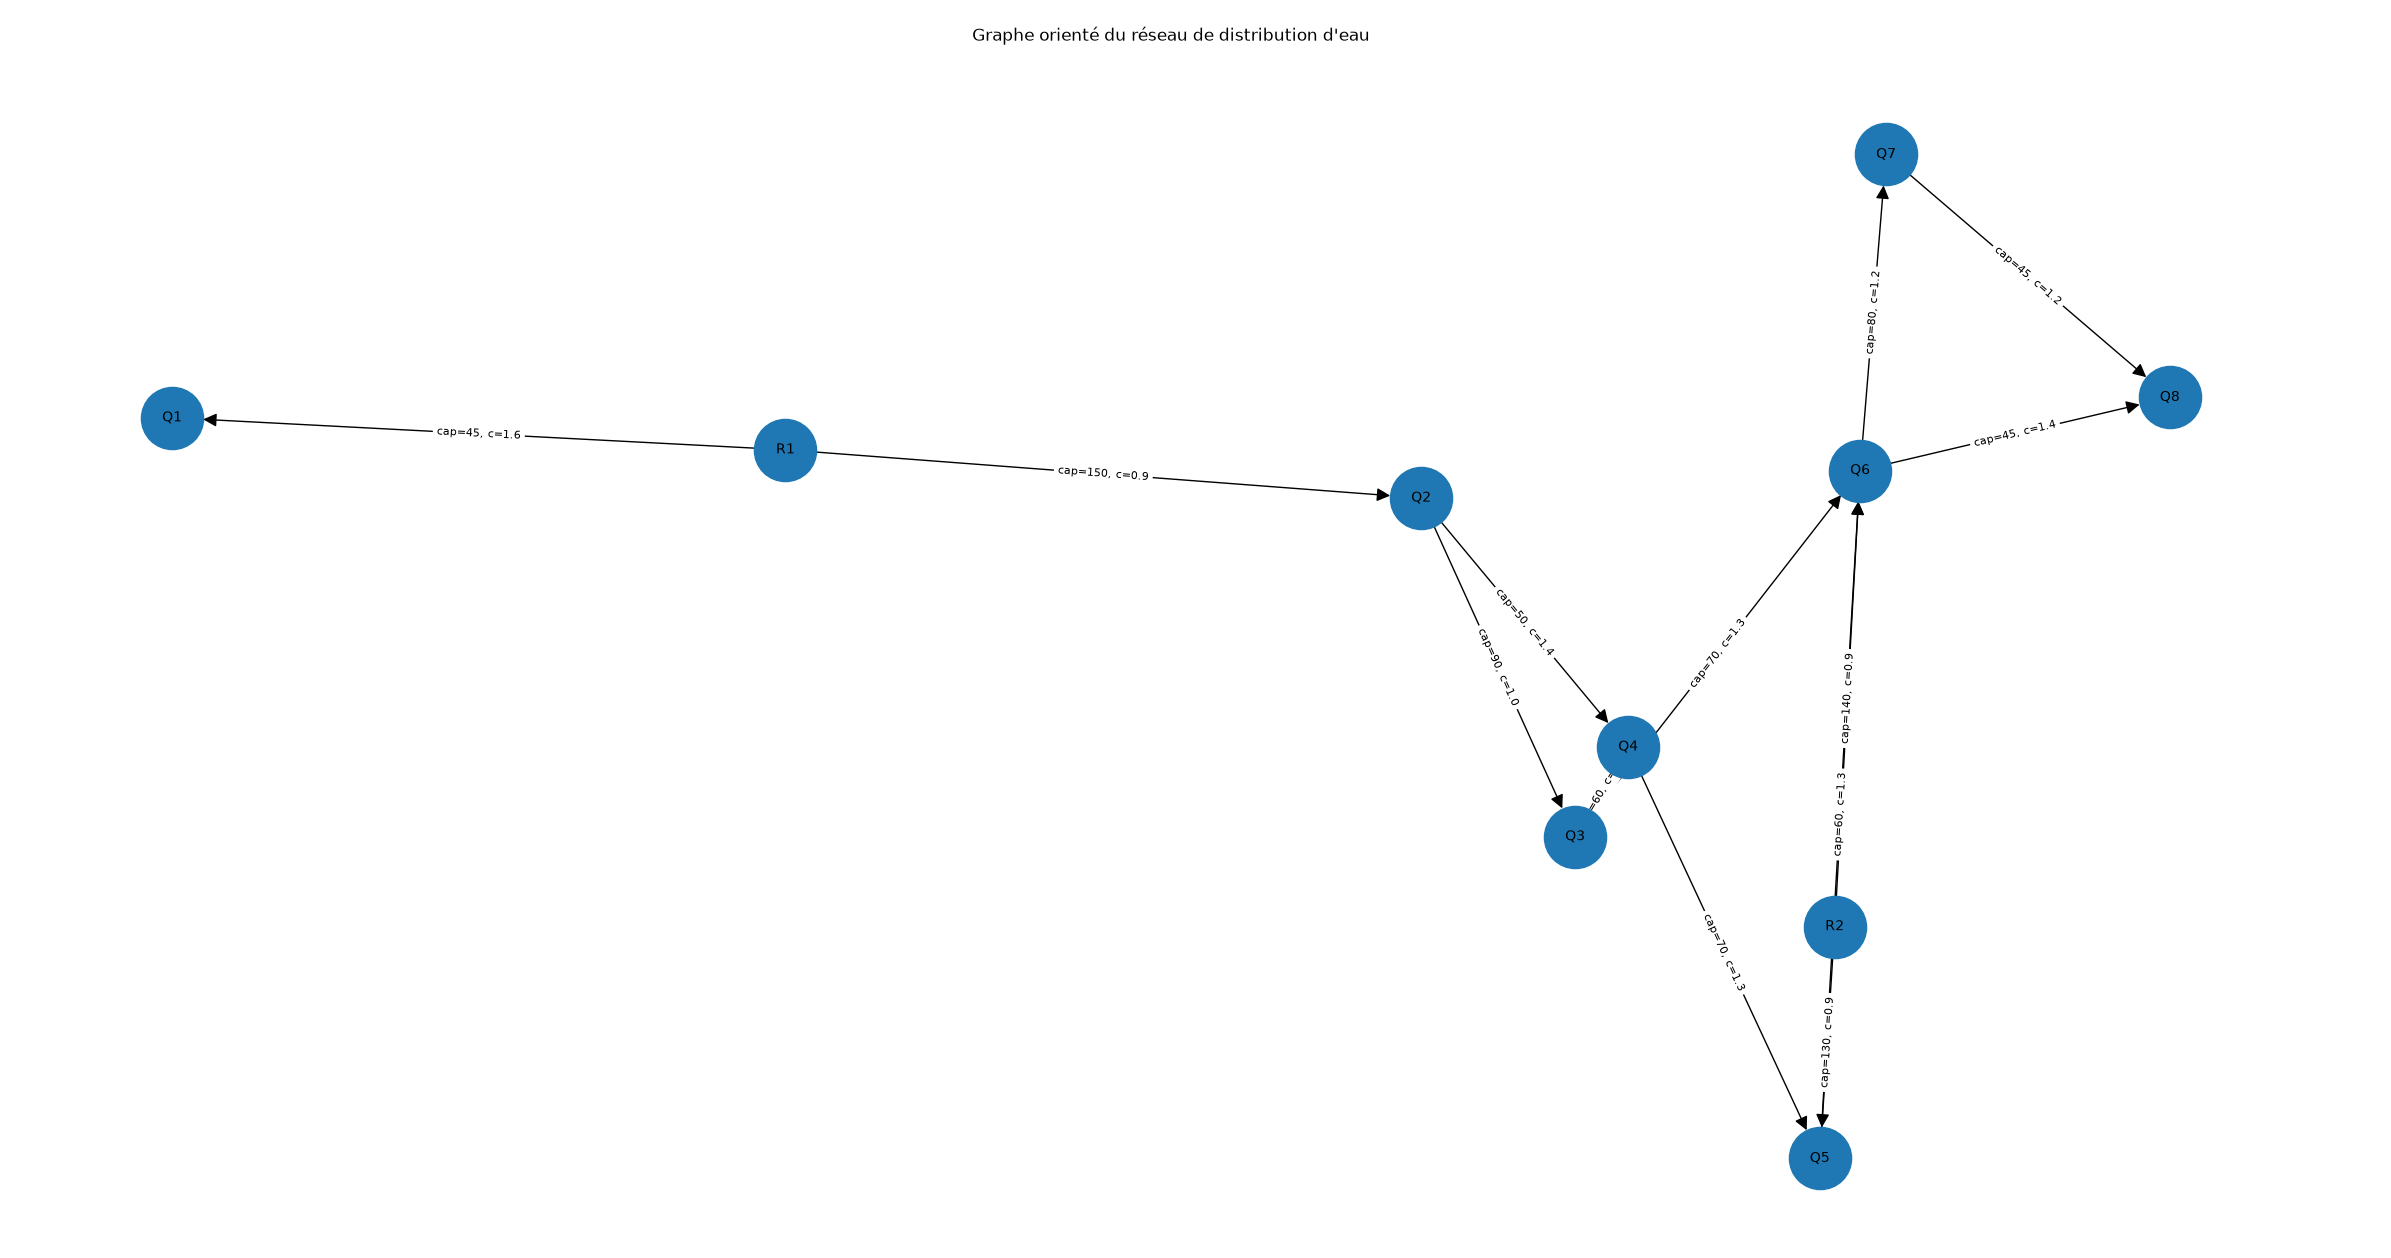
\includegraphics[width=\textwidth, trim={4cm 1cm 4cm 1cm}, clip]{graphe_reseau.png}
\caption{Représentation topologique orientée du réseau d'eau, illustrant les réservoirs $\{R_1, R_2\}$, les quartiers $\{Q_1, \dots, Q_8\}$, les arêtes-ponts vers $Q_1$ et la redondance maillée de la zone aval.}
\label{fig:topologie-visuelle}
\end{figure}
\end{document}

